\documentclass[../main]{subfiles}

\questiontrue
\solutiontrue

\begin{document}
    \ifquestion

\section{Black Holes}

After many years, the parent star of the Kafshian stellar system enters a supernova state and becomes a black hole. Fortunately, the civilization managed to escape centuries before this event, and you, an inhabitant of the Kafsh II system, wish to study more about the history of your ancestors and, consequently, learn more about black holes and general relativity!

\parte{A}{Metrics}

First, we need a way to describe the space-time around us. For this, we can define metrics capable of describing the curvature of space-time due to the presence of matter. To do this, we will define the concept of an interval $ds$ between two events $A$ and $B$ for flat space-time (infinitely distant from any mass):

\[(\text{interval})^2 = (\text{distance traveled by light in the time interval})^2 - (\text{distance between events } A \text{ and } B)^2\]

Or:

\[(ds)^2 = (cdt)^2 - (dx)^2 - (dy)^2 - (dz)^2\]

However, in the following problems, the spatial description will be easier if we use spherical coordinates instead of Cartesian coordinates.

\ut{A.1} Demonstrate the definition of the interval using spherical coordinates $(r, \theta, \phi)$.

\begin{doublespace}

\end{doublespace}

For $(ds)^2 > 0$, the value of $(cdt)^2$ dominates, meaning that light has more than enough time to travel between events. For $(ds)^2 = 0$, only light can travel between events $A$ and $B$. For $(ds)^2 < 0$, as expected, not even light can access events $A$ and $B$.

By definition, the time between two events occurring at the same spatial coordinate is called proper time:

\[\delta \tau = \frac{\delta s}{c}\]

On the other hand, the distance between two events occurring at the same temporal coordinate is called proper distance:

\[\delta L = \sqrt{-(\delta s)^2}\]

When dealing with space-time that may be curved due to the presence of matter, the trajectory of a body—or even light—can be described using the concept of the interval. The trajectory of a freely falling body is defined as a geodesic of maximum interval, and the trajectory of light is defined as a geodesic of zero interval!

In 1916, the German physicist Schwarzschild solved Einstein's field equations and obtained a metric that describes space-time around\footnote{The equations are valid only outside the body.} a single body with mass $M$ and radius $R$:

\[(ds)^2 = \left(cdt \sqrt{1 - \frac{2GM}{rc^2}}\right)^2 - \left(\frac{dr}{\sqrt{1 - \frac{2GM}{rc^2}}}\right)^2 - (rd\theta)^2 - (r\sin(\theta)d\phi)^2\]

However, be careful! A common mistake is to consider that $r$ is the distance between the center of the body and the point being analyzed. The value of $r$ simply represents the spatial coordinate of the point. To calculate the actual distance, relativistic effects that alter the proper distance must be considered (unlike in special relativity, the proper distance varies with respect to the coordinate $r$). This also means that the variables in the metric are those observed from an observer at an infinite distance from the body (essentially outside the curvature).

\ut{A.2} For this metric, find the values of $\Delta L(r_1 \rightarrow r_2)$ (measured radially) and $\Delta \tau(t_1 \rightarrow t_2)$. If necessary, use:

\[\int \frac{dx}{\sqrt{1 - \frac{a}{x}}} = x\sqrt{1 - \frac{a}{x}} + a\tanh^{-1}\left(\sqrt{1 - \frac{a}{x}}\right) + C\]

\ut{A.3} Consider a radiation jet with frequency $\nu_0$ emitted radially from a spatial coordinate $r$. Find the frequency $\nu_\infty$ received by an external observer, considering only gravitational redshift. Hint: remember that frequency is inversely proportional to the period between two oscillations.

\ut{A.4} Now, we would like to analyze a circular orbit around the object. Resist the urge to use Newtonian physics and follow Schwarzschild’s metric to find the angular velocity $\omega$ of the orbit.

\parte{B}{Black Holes}

\ut{B.1} For some objects in the universe, the curvature in space-time caused by their existence is such that not even light can "escape" their attraction. Conveniently, we call these objects Black Holes! Find the relation for the radius $R$ of this limit, called the Event Horizon.

\ut{B.2} Find the value of $r$ for which a photon would describe a circular orbit around the black hole. The set of points with such a coordinate is called the Photon Sphere.

\ut{B.3} In some cases in general relativity, it is still possible to use Newtonian physics with slight corrections. The equation that determines the attractive "force"\footnote{In this case, this "force" is more related to the effective potential energy than to an actual force acting on the body.} of a test body $m$ at a distance $r$ from the central body $M$ with angular momentum $L$ is:

\[|\vec{F}| = \frac{GMm}{r^2} + \frac{3GML^2}{mc^2r^4}\]

Find the expression for the radius of the innermost stable circular orbit (\textit{Innermost Stable Circular Orbit}, $r_{ISCO}$) with angular momentum $L$. Hint: Initially treat $L$ as a fixed value, then make the necessary considerations.

\begin{doublespace}

\end{doublespace}

Another very useful metric (with broader applicability) is the Kerr metric, which deals with black holes with non-zero \textit{spin}. Unlike in quantum mechanics, here \textit{spin} literally means the rotation of the black hole. It makes sense to think that black holes have \textit{spin} because stars initially have angular momentum that must be preserved. In these cases, we can describe the rotation of the black hole using a spin parameter represented by $a_*$, which can vary from $-1$ to $1$, with $1$ being the maximum rotation allowed by the \textit{Cosmic Censorship Hypothesis}, which rules out the existence of naked singularities. In this metric, one can develop the equation that relates $r_{ISCO}$ to the spin parameter $a_*$:

\[r_{ISCO} = \frac{GM}{c^2}\left(1 + \sqrt{8.354\left((2 - a_*)^2 - 1\right)}\right)\]

\ut{B.4} One technique to determine $a_*$ is through the analysis of the observed frequency of the iron $K_\alpha$ emission lines near $r_{ISCO}$. You, a scientist from the Kafsh II system, observe a sample of the emission spectrum from the accretion disk of the black hole $M33\, X-7$, with a mass of $M_{M33X-7} = (15.65 \pm 1.45)M_\odot$, which has a companion star in a binary system. You notice that the minimum received $K_\alpha$ frequency was $\nu = 7.83 \cdot 10^{17}\,Hz$. For simplicity, we will use the approximation (which is invalid in this case, as it is a rotating black hole) obtained in item \textbf{A.3)}. Determine the spin parameter of this black hole. Consider that the iron $K_\alpha$ transition energy is $E_{FeK\alpha} = 6.38\,KeV$.

\parte{C}{“Black” Thermodynamics}

As proposed by Stephen Hawking, the temperature of a black hole can be expressed as:

\[T_b = \frac{\hbar c^3}{8 \pi GMk_b}\]

\ut{C.1} Thus, find the emission power of a black hole acting as a blackbody.

\ut{C.2} Consider that for a body at rest, $E = Mc^2$. What is the estimated lifetime of this black hole?

\begin{doublespace}

\end{doublespace}

It is believed that a black hole has an associated entropy because, if $S = 0$ in any case, it would be terrifyingly possible for the universe’s entropy to decrease as matter is absorbed by the black hole.

\ut{C.3} Knowing that $dS = \frac{dQ}{T}$ (the classical thermodynamic interpretation of entropy), what should be the entropy of a black hole?


	\clearpage
    
    
    \fi
    
    \ifsolution
    
    \section{Black Holes}
	
	\parte{A}{Metrics}
	
	\ut{A.1} Consider what it is shown on the Figure \ref{fig:mito}.
	
	\begin{figure}[htpb]
	    \centering
	    
\tikzset{every picture/.style={line width=0.75pt}} %set default line width to 0.75pt        

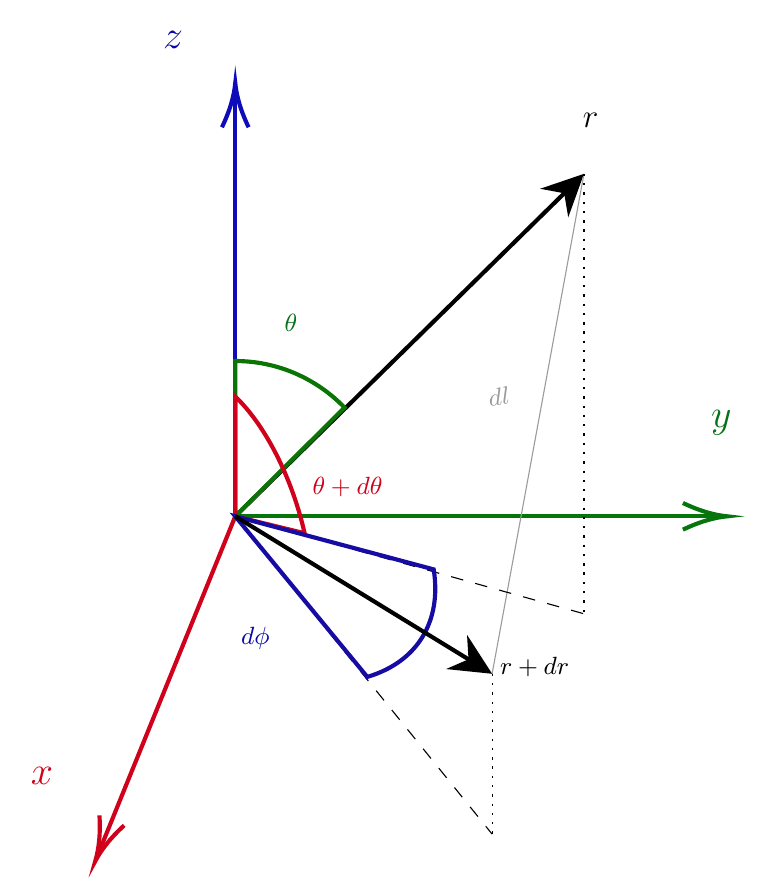
\begin{tikzpicture}[x=0.75pt,y=0.75pt,yscale=-1.5,xscale=1.5]
%uncomment if require: \path (0,542); %set diagram left start at 0, and has height of 542

%Straight Lines [id:da6210423395523805] 
\draw [color={rgb, 255:red, 14; green, 12; blue, 186 }  ,draw opacity=1 ][line width=1.5]    (283,203.17) -- (283,339.34) ;
\draw [shift={(283,200.17)}, rotate = 90] [color={rgb, 255:red, 14; green, 12; blue, 186 }  ,draw opacity=1 ][line width=1.5]    (14.21,-4.28) .. controls (9.04,-1.82) and (4.3,-0.39) .. (0,0) .. controls (4.3,0.39) and (9.04,1.82) .. (14.21,4.28)   ;
%Straight Lines [id:da019548336065443594] 
\draw [color={rgb, 255:red, 5; green, 117; blue, 12 }  ,draw opacity=1 ][line width=1.5]    (283,339.34) -- (438,339.34) ;
\draw [shift={(441,339.34)}, rotate = 180] [color={rgb, 255:red, 5; green, 117; blue, 12 }  ,draw opacity=1 ][line width=1.5]    (14.21,-4.28) .. controls (9.04,-1.82) and (4.3,-0.39) .. (0,0) .. controls (4.3,0.39) and (9.04,1.82) .. (14.21,4.28)   ;
%Straight Lines [id:da5222422439312144] 
\draw [color={rgb, 255:red, 208; green, 2; blue, 27 }  ,draw opacity=1 ][line width=1.5]    (283,339.34) -- (239.13,447.39) ;
\draw [shift={(238,450.17)}, rotate = 292.1] [color={rgb, 255:red, 208; green, 2; blue, 27 }  ,draw opacity=1 ][line width=1.5]    (14.21,-4.28) .. controls (9.04,-1.82) and (4.3,-0.39) .. (0,0) .. controls (4.3,0.39) and (9.04,1.82) .. (14.21,4.28)   ;
%Straight Lines [id:da9228333288264807] 
\draw [line width=1.5]    (283,339.34) -- (392.15,232.15) ;
\draw [shift={(395,229.34)}, rotate = 135.52] [fill={rgb, 255:red, 0; green, 0; blue, 0 }  ][line width=0.08]  [draw opacity=0] (13.4,-6.43) -- (0,0) -- (13.4,6.44) -- (8.9,0) -- cycle    ;
%Straight Lines [id:da9748339892315263] 
\draw [color={rgb, 255:red, 155; green, 155; blue, 155 }  ,draw opacity=1 ]   (395,229.34) -- (365.5,389.92) ;
%Shape: Pie [id:dp8167850161158197] 
\draw  [color={rgb, 255:red, 10; green, 117; blue, 5 }  ,draw opacity=1 ][line width=1.5]  (283,289.46) .. controls (283,289.46) and (283,289.46) .. (283,289.46) .. controls (283,289.46) and (283,289.46) .. (283,289.46) .. controls (296.74,289.46) and (309.17,295.19) .. (318.09,304.41) -- (283,339.34) -- cycle ;
%Shape: Pie [id:dp6891764194445413] 
\draw  [color={rgb, 255:red, 208; green, 2; blue, 27 }  ,draw opacity=1 ][line width=1.5]  (283,300.88) .. controls (290.04,307.56) and (297.02,318.96) .. (301.83,332.78) .. controls (303.25,336.85) and (304.39,340.88) .. (305.27,344.78) -- (283,339.34) -- cycle ;
%Straight Lines [id:da7281869622246289] 
\draw  [dash pattern={on 4.5pt off 4.5pt}]  (283,339.34) -- (396,370.92) ;
%Straight Lines [id:da8866690597125835] 
\draw  [dash pattern={on 4.5pt off 4.5pt}]  (283,339.34) -- (365.5,441.42) ;
%Shape: Pie [id:dp3477850655358974] 
\draw  [color={rgb, 255:red, 22; green, 11; blue, 162 }  ,draw opacity=1 ][line width=1.5]  (346.73,356.39) .. controls (349.39,373.11) and (341.46,386.17) .. (325.4,390.92) -- (283,339.34) -- cycle ;
%Straight Lines [id:da4156785752738812] 
\draw [line width=1.5]    (283,339.34) -- (362.09,387.83) ;
\draw [shift={(365.5,389.92)}, rotate = 211.51] [fill={rgb, 255:red, 0; green, 0; blue, 0 }  ][line width=0.08]  [draw opacity=0] (13.4,-6.43) -- (0,0) -- (13.4,6.44) -- (8.9,0) -- cycle    ;
%Straight Lines [id:da6554847125958474] 
\draw  [dash pattern={on 0.84pt off 2.51pt}]  (395,229.34) -- (395,370.92) ;
%Straight Lines [id:da6452597633307695] 
\draw  [dash pattern={on 0.84pt off 2.51pt}]  (365.5,389.92) -- (365.5,441.42) ;

% Text Node
\draw (259,182.57) node [anchor=north west][inner sep=0.75pt]  [font=\Large,color={rgb, 255:red, 7; green, 8; blue, 167 }  ,opacity=1 ]  {$z$};
% Text Node
\draw (216.5,419.07) node [anchor=north west][inner sep=0.75pt]  [font=\Large,color={rgb, 255:red, 208; green, 2; blue, 27 }  ,opacity=1 ]  {$x$};
% Text Node
\draw (435,304.57) node [anchor=north west][inner sep=0.75pt]  [font=\Large,color={rgb, 255:red, 7; green, 113; blue, 23 }  ,opacity=1 ]  {$y$};
% Text Node
\draw (298,273.57) node [anchor=north west][inner sep=0.75pt]  [font=\small,color={rgb, 255:red, 7; green, 113; blue, 23 }  ,opacity=1 ]  {$\theta $};
% Text Node
\draw (307,326) node [anchor=north west][inner sep=0.75pt]  [font=\small,color={rgb, 255:red, 208; green, 2; blue, 27 }  ,opacity=1 ]  {$\theta +d\theta $};
% Text Node
\draw (393.83,209.07) node [anchor=north west][inner sep=0.75pt]  [font=\large]  {$r$};
% Text Node
\draw (367.22,383.75) node [anchor=north west][inner sep=0.75pt]  [font=\small]  {$r+dr$};
% Text Node
\draw (363.06,297.69) node [anchor=north west][inner sep=0.75pt]  [font=\small,color={rgb, 255:red, 155; green, 155; blue, 155 }  ,opacity=1 ,rotate=-353.56]  {$dl$};
% Text Node
\draw (284,374.07) node [anchor=north west][inner sep=0.75pt]  [font=\small,color={rgb, 255:red, 7; green, 8; blue, 167 }  ,opacity=1 ]  {$d\phi $};


\end{tikzpicture}
	    \caption{Applied spherical coordinates}
	    \label{fig:mito}
	\end{figure}
	
    Notice that $(dx)^2+(dy)^2+(dz)^2=(dl)^2$, by the Pythagorean Theorem. Therefore we want to determine $(dl)^2$ in terms of the spherical coordinates. In order to do so, we can use the approximation for infinitesimal segments, as shown in the figure \ref{fig:brasilbestcountry}:
	
	\begin{figure}[htpb]
	    \centering
	    

\tikzset{every picture/.style={line width=0.75pt}} %set default line width to 0.75pt        

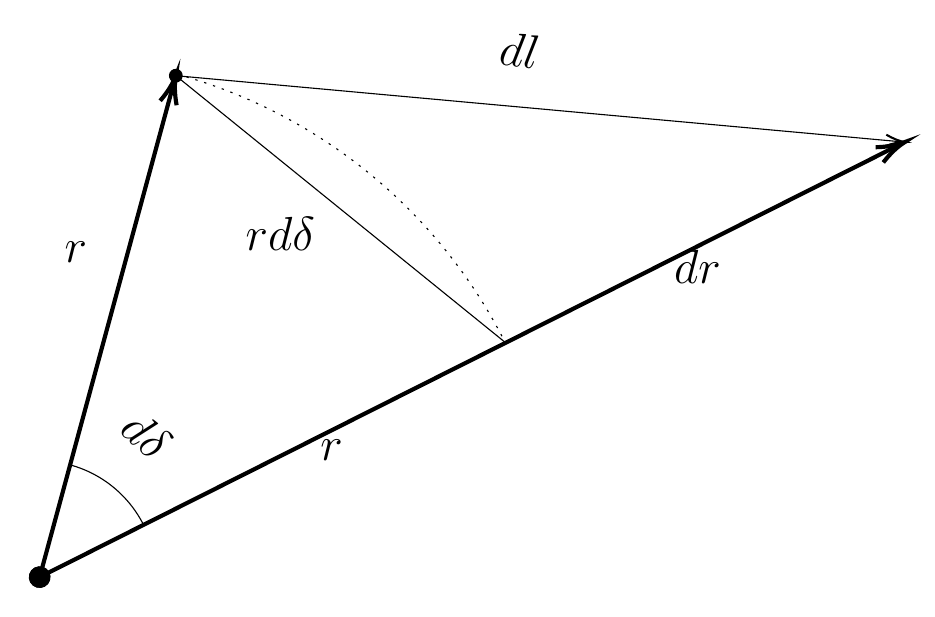
\begin{tikzpicture}[x=0.75pt,y=0.75pt,yscale=-1.2,xscale=1.2]
%uncomment if require: \path (0,542); %set diagram left start at 0, and has height of 542

%Straight Lines [id:da6493340895042639] 
\draw [line width=1.5]    (238.33,409.34) -- (292.21,210.91) ;
\draw [shift={(293,208.01)}, rotate = 105.19] [color={rgb, 255:red, 0; green, 0; blue, 0 }  ][line width=1.5]    (11.37,-3.42) .. controls (7.23,-1.45) and (3.44,-0.31) .. (0,0) .. controls (3.44,0.31) and (7.23,1.45) .. (11.37,3.42)   ;
\draw [shift={(238.33,409.34)}, rotate = 285.19] [color={rgb, 255:red, 0; green, 0; blue, 0 }  ][fill={rgb, 255:red, 0; green, 0; blue, 0 }  ][line width=1.5]      (0, 0) circle [x radius= 3.48, y radius= 3.48]   ;
%Straight Lines [id:da24688574092848503] 
\draw [line width=1.5]    (238.33,409.34) -- (582.99,236.02) ;
\draw [shift={(585.67,234.68)}, rotate = 153.3] [color={rgb, 255:red, 0; green, 0; blue, 0 }  ][line width=1.5]    (11.37,-3.42) .. controls (7.23,-1.45) and (3.44,-0.31) .. (0,0) .. controls (3.44,0.31) and (7.23,1.45) .. (11.37,3.42)   ;
\draw [shift={(238.33,409.34)}, rotate = 333.3] [color={rgb, 255:red, 0; green, 0; blue, 0 }  ][fill={rgb, 255:red, 0; green, 0; blue, 0 }  ][line width=1.5]      (0, 0) circle [x radius= 3.48, y radius= 3.48]   ;
%Straight Lines [id:da6600105484470336] 
\draw    (293,208.01) -- (583.67,234.5) ;
\draw [shift={(585.67,234.68)}, rotate = 185.21] [color={rgb, 255:red, 0; green, 0; blue, 0 }  ][line width=0.75]    (7.65,-2.3) .. controls (4.86,-0.97) and (2.31,-0.21) .. (0,0) .. controls (2.31,0.21) and (4.86,0.98) .. (7.65,2.3)   ;
\draw [shift={(293,208.01)}, rotate = 5.21] [color={rgb, 255:red, 0; green, 0; blue, 0 }  ][fill={rgb, 255:red, 0; green, 0; blue, 0 }  ][line width=0.75]      (0, 0) circle [x radius= 2.34, y radius= 2.34]   ;
%Shape: Arc [id:dp44405338873426703] 
\draw  [draw opacity=0][dash pattern={on 0.84pt off 2.51pt}] (293.7,207.5) .. controls (351.18,223.23) and (398.79,262.86) .. (425.18,315.04) -- (238.33,409.34) -- cycle ; \draw  [dash pattern={on 0.84pt off 2.51pt}] (293.7,207.5) .. controls (351.18,223.23) and (398.79,262.86) .. (425.18,315.04) ;  
%Shape: Arc [id:dp04791890377613761] 
\draw  [draw opacity=0] (250.69,364.31) .. controls (263.51,367.82) and (274.13,376.66) .. (280.02,388.31) -- (238.33,409.34) -- cycle ; \draw   (250.69,364.31) .. controls (263.51,367.82) and (274.13,376.66) .. (280.02,388.31) ;  
%Straight Lines [id:da4620126806652938] 
\draw    (293,208.01) -- (425.18,315.04) ;

% Text Node
\draw (247.33,273.74) node [anchor=north west][inner sep=0.75pt]  [font=\LARGE]  {$r$};
% Text Node
\draw (350,353) node [anchor=north west][inner sep=0.75pt]  [font=\LARGE]  {$r$};
% Text Node
\draw (279.23,339.56) node [anchor=north west][inner sep=0.75pt]  [font=\LARGE,rotate=-43.27]  {$d\delta $};
% Text Node
\draw (423.32,188.96) node [anchor=north west][inner sep=0.75pt]  [font=\LARGE,rotate=-7.19]  {$dl$};
% Text Node
\draw (492,277.08) node [anchor=north west][inner sep=0.75pt]  [font=\LARGE]  {$dr$};
% Text Node
\draw (320,264) node [anchor=north west][inner sep=0.75pt]  [font=\LARGE]  {$rd\delta $};


\end{tikzpicture}
	    \caption{Infinitesimal variation on the position vector with the angle}
	    \label{fig:brasilbestcountry}
	\end{figure}
	
    \[(dl)^2=r^2(d\delta)^2+(dr)^2\]
	
	In order to calculate the angle $d\delta$, between the two vectors, podemos utilizar a lei dos cossenos na trigonometria esférica, de tal forma que:
	
	\[\cos{(d\delta)}=\cos{(\theta)}\cos{(\theta+d\theta)}+\sin{(\theta)}\sin{(\theta+d\theta)}\cos{(d\phi)}\]

	You might be tempted to use approximations like \(\cos(dx) = 1\) or even \(\cos(\theta + d\theta) = \cos(\theta) - \sin(\theta) d\theta\). However, all these approximations ignore terms of order \(d\delta^2\), \(d\theta^2\), and \(d\phi^2\), which should not be neglected in this case, as these are precisely the terms we need to describe \(dl^2\). Therefore, we will have to make approximations that preserve such terms, using \(\cos(dx) = 1 - \frac{dx^2}{2}\), and we will need to apply the sum formulas for sine and cosine.
	
	
	\[1-\frac{d\delta^2}{2}=\cos{(\theta)}\left( \cos{(\theta)}\left( 1-\frac{d\theta^2}{2}\right)-\sin{(\theta)}d\theta \right)\]
	
	\[+\sin{(\theta)}\left(\sin{(\theta)} \left(1-\frac{d\theta^2}{2} \right)+\cos{(\theta)}d\theta \right)\left(1-\frac{d\phi^2}{2} \right)   \]

After all the necessary simplifications and the exclusion of third-order terms, we find that:  

\[
d\delta^2 = d\theta^2 + \sin^2(\theta) d\phi^2
\]  

Thus, substituting into the expression for distance, we obtain:  

\[
(dl)^2 = (r d\theta)^2 + (r \sin(\theta) d\phi)^2 + (dr)^2
\]  

Hence, we have proven that the expression for the metric in flat spacetime, in its polar form, is:  

\[
(ds)^2 = (c dt)^2 - (r d\theta)^2 - (r \sin(\theta) d\phi)^2 - (dr)^2
\]  

\ut{A.2} By the given definition, the calculation of \(\Delta L\) implies an instantaneous measurement, meaning \(dt = 0\) and, since it is radial, \(d\theta = 0\) and \(d\phi = 0\):  

\[
(ds)^2 = -\left( \frac{dr}{\sqrt{1 - \frac{2GM}{r c^2}}} \right)^2
\]  

Since \(dL = \sqrt{-(ds)^2}\), we find that:  

\[
dL = \frac{dr}{\sqrt{1 - \frac{2GM}{r c^2}}}
\]  

\[
\rightarrow \int dL = \int_{r_1}^{r_2} \frac{dr}{\sqrt{1 - \frac{2GM}{r c^2}}}
\]  

Using the integral provided in the problem statement:  

\[
\Delta L = r_2 \sqrt{1 - \frac{2GM}{r_2 c^2}} + \frac{2GM}{c^2} \tanh^{-1} \left( \sqrt{1 - \frac{2GM}{r_2 c^2}} \right) - r_1 \sqrt{1 - \frac{2GM}{r_1 c^2}} + \frac{2GM}{c^2} \tanh^{-1} \left( \sqrt{1 - \frac{2GM}{r_1 c^2}} \right)
\]  

For the proper time, by definition, we know that in this analysis the spatial coordinates remain constant, implying:  

\[
(ds)^2 = \left( c dt \sqrt{1 - \frac{2GM}{r c^2}} \right)^2
\]  

\[
\therefore \Delta \tau = \sqrt{1 - \frac{2GM}{r c^2}} \, \Delta t
\]  

\ut{A.3} It is known that \(\nu \propto T^{-1}\), where \(T\) is the oscillation period of the electromagnetic wave. Thus:  

\[
\frac{T_0}{T_\infty} = \frac{\nu_\infty}{\nu_0}
\]  

Using the relation from the previous item\footnote{Remember that the definition of \(dt\) refers to the time interval observed by an observer outside the spacetime curvature, as it is the temporal coordinate.}, we can relate:  

\[
T_0 = \sqrt{1 - \frac{2GM}{r c^2}} \, T_\infty
\]  

Hence:  

\[
\nu_\infty = \nu_0 \sqrt{1 - \frac{2GM}{r c^2}}
\]  

\ut{A.4} Assume a circular orbit located in the equatorial plane of the coordinate system, so that \(\theta = \frac{\pi}{2}\) and \(d\phi = \omega dt\). Thus, we know that \(dr = d\theta = 0\):  

\[
(ds)^2 = \left( c dt \sqrt{1 - \frac{2GM}{r c^2}} \right)^2 - (r \omega dt)^2
\]  

Simplifying the expression, we obtain the interval for an orbit as:  

\[
\Delta s = \int_0^{\frac{2\pi}{\omega}} \sqrt{c^2 - \frac{2GM}{r} - r^2 \omega^2} \, dt
\]  

In the case of a free orbit without external forces, the body will follow the path with the smallest possible interval. Thus, we determine the value of \(r\) that provides this minimum:  

\[
\frac{d}{dr} \Delta s = \int_0^{\frac{2\pi}{\omega}} \frac{d}{dr} \sqrt{c^2 - \frac{2GM}{r} - r^2 \omega^2} \, dt = 0
\]  

For this, we require:  

\[
\frac{d}{dr} \left( \frac{2GM}{r} + r^2 \omega^2 \right) = 0
\]  

Solving, we find that, "coincidentally," the result matches the prediction from Newtonian physics:  

\[
\omega = \sqrt{\frac{GM}{r^3}}
\]  


\parte{B}{Black Holes}

\ut{B.1} In this situation, light does not make progress (does not move) in the spatial coordinates, as it is "trapped," so $dr=d\theta=d\phi=0$, and furthermore, since we know that it must always move along a null geodesic: $ds=0$. Therefore:

\[cdt\sqrt{1-\frac{2GM}{rc^2}}=0\]

Since there is no restriction on its temporal coordinate, it is understood that $dt \ne 0$, hence:

\[r=\frac{2GM}{c^2}\]

Which is the same result obtained by the Newtonian prediction!

\ut{B.2} In this case, using the same convention as in \textbf{A.4)}, it is known that $dr=d\theta=ds=0$, $\sin{(\theta)}=1$, and that $d\phi=\omega dt$. Note also that the result of item \textbf{A.4)} is not restricted to massive particles, since light also moves along a geodesic such that $\dfrac{d}{dr}\Delta s = 0$ (which is obvious, since $\Delta s$ is essentially $0$), so we can directly substitute the value of $\omega$ found:

\[cdt\sqrt{1-\frac{2GM}{rc^2}}=r\sqrt{\frac{GM}{r^3}}dt\]

Thus, we find that:

\[r=\frac{3GM}{c^2}\]

\ut{B.3} Equating the gravitational force to the centripetal force ($v=\dfrac{L}{mr}$):

\[\frac{GMm}{r^2}+\frac{3GML^2}{mc^2r^4}=\frac{L^2}{mr^3}\]

Rearranging, we find that:

\[r^2-\frac{L^2}{GMm^2}r+3\frac{L^2}{m^2c^2}=0\]

Solving for $r$:

\[r=\frac{L^2}{2GMm^2}\left( 1 \pm \sqrt{1-\frac{12G^2M^2m^2}{L^2c^2}}\right) \]

Note that in the case where we return to classical physics by making $c\rightarrow\infty$, it is expected that we find the classical result. When we do this, the solution with the minus sign shows that $r\rightarrow0$ when $c\rightarrow\infty$, so it is understood that the stable orbit is:

\[r=\frac{L^2}{2GMm^2}\left( 1 + 
    \sqrt{1-\frac{12G^2M^2m^2}{L^2c^2}}\right) \]

Note that to have a minimum $r$, we need $L$ to also be minimum. Therefore, respecting the existence condition for the square root, we will set $L^2=\dfrac{12G^2M^2m^2}{c^2}$:

\[r=\frac{12G^2M^2m^2}{2GMm^2c^2}\]

\[r_{ISCO}=\frac{6GM}{c^2}\]

\ut{B.4} Note that the minimum frequency is the one that has undergone the maximum possible redshift, so it is the one that departed from $r_{ISCO}$. It is known that the rest frequency of the emission line can be found as: $E_{FeK\alpha}=h\nu_0$, which gives us the data: $\nu_0=1.539\cdot 10^{18}Hz$. From the gravitational redshift equation:

\[7.83\cdot10^{17}Hz=1.539\cdot 10^{18}\sqrt{1-\frac{2GM}{r_{ISCO}c^2}}\] 

Substituting the data, we find that $r_{ISCO}=2.7\dfrac{GM}{c^2}$. Note that there is no need to substitute the mass of the black hole, because we can now conclude that:

\[1+ \sqrt{8.354\left( (2-a_*)^2-1\right) }=2.7\]

Finally, we find that:

\[a_*=0.84\]

\parte{C}{"Black" Thermodynamics}

\ut{C.1} Starting from the proposed temperature relation, we can find a relation for the "luminosity" (it does not mean light emission, since the hole is black) using the same Stefan-Boltzmann relation:

\[P_b=4 \pi R_b^2 \sigma T_b^4\]

Where $R_b$ is the radius of the event horizon of the star, given by the Schwarzschild relation:

\[R_b = \frac{2GM}{c^2}\]

Therefore, we have:

\[P_b = 4 \pi \left( \frac{2GM}{c^2}\right)^2 \sigma \left(\frac{\hbar c^3}{8 \pi GMk_b}\right)^4\]

Simplifying:

\[P_b = \frac{\hbar^4 c^8 \sigma}{256 \pi^3 G^2 M^2 k_b^4}\]

\ut{C.2} Where does this energy being released come from? From the black hole's own mass (as defined by the model in the statement), so we have that $E_b = Mc^2$ and, for small energy variations: $\Delta E_b = \Delta M c^2$, or, analyzing infinitesimal variations: $d E_b = d M c^2$.
Note that the energy released in an interval $dt$ will be $P_bdt$, so we will have:

\[P_bdt=-dE_b=-dMc^2\]

The negative sign is used because there is energy release (decrease in the internal energy of the black hole)

\[\frac{\hbar^4 c^8 \sigma}{256 \pi^3 G^2 M^2 k_b^4}dt=-dMc^2\]

Rearranging:

\[\frac{\hbar^4 c^6 \sigma}{256 \pi^3 G^2 k_b^4}dt=-M^2dM\]

Integrating the expression, we have:

\[\frac{\hbar^4 c^6 \sigma}{256 \pi^3 G^2 k_b^4}(t-t_0)=-\left(\frac{M^3}{3}-\frac{M_0^3}{3}\right)\]	

Where $t_0$ is the initial time (t=0) and $M_0$ is the initial mass, so the black hole "dies" when it is completely evaporated, that is, $M=0$. Thus, we have:

\[\frac{\hbar^4 c^6 \sigma}{256 \pi^3 G^2 k_b^4}(\Delta t)=-\left(\frac{0^3}{3}-\frac{M_0^3}{3}\right)\]	

\[\therefore \Delta t=\left(\frac{256 \pi^3 G^2 k_b^4 M_0^3}{3 \hbar^4 c^6 \sigma}\right)\]	

Bonus: Lifetime of a black hole with the mass of the Sun: $2.1 \cdot 10^{67}$ years.

\ut{C.3} Note that we already have an expression for the emitted power and we know that $dMc^2 = dQ$, so:

\[dS = dMc^2 \frac{1}{T} = dM c^2 \frac{8 \pi GMk_b}{\hbar c^3}\]

Integrating, we will have:

\[S-S_0=\frac{4 \pi GM^2k_b}{\hbar c} - \frac{4 \pi GM_0^2k_b}{\hbar c}\]

Thus, we associate:

\[S=\frac{4 \pi GM^2k_b}{\hbar c}\]
	
	
	\clearpage
    
    
    \fi
\end{document}
